\paragraph{}
Pour valider la réalisation des besoins fonctionnels et non fonctionnels présentés dans le cahier des charges, une série de tests a été effectuée sur le logiciel.

\paragraph{}
Concernant les besoins fonctionnels, nous avons manipulé le logiciel sous les différents systèmes d'exploitation envisagés, à savoir Windows et Linux.
Les différentes rotations de la caméra autour de la scène ont bien été implémentées, permettant à l'utilisateur de voir les objets qui y sont placés sous différents angles, et de s'en rapprocher ou de s'en éloigner grâce au zoom. La translation de la caméra a également été implémentée, même si son utilisation nécessite une souris.
Les objets sont issus de fichiers d'extension OBJ version 3.0, ASCII, ou PLY, versions 1.0, ASCII et binaire. Ceux-ci peuvent ensuite être sélectionnés un par un, en cliquant sur la scène ou sur son nom dans la liste des objets. L'utilisateur peut alors les déplacer grâce à des translations et rotations selon trois axes, et modifier leur taille. Ils pourront également être supprimés de la scène.
Enfin, les différents rendus prévus ont pu être obtenus à partir de la scène. Pour chacun d'entre eux, une nouvelle fenêtre est ouverte, proposant les paramètres modifiables pour la génération des photographies, anaglyphes, autostéréogrammes, et folioscopes. Pour chacun d'entre eux, on proposera une prévisualisation, et la possibilité d'enregistrer les images intermédiaires ayant permis ce résultat, à savoir les vues gauche et droite pour les anaglyphes, la carte des profondeurs pour les autostéréogrammes, et chaque image du folioscope permettant d'obtenir un GIF animé.
Comme prévu, même si l'utilisateur ne demande pas d'enregistrer la scène, une sauvegarde automatique a été mise en place à intervalles de temps régulier. Elle permet de s'assurer que même en cas d'arrêt non souhaité du logiciel, seules les dernières modifications seront perdues.

\paragraph{}
Les tests des besoins non fonctionnels ont permis de valider la portabilité et la fluidité du logiciel. L'extensibilité du logiciel aura été permise par l'architecture du logiciel, qui a été présentée dans la partie Réalisation du projet.
Pour s'assurer de la portabilité du logiciel, nous avons manipulé le logiciel sous les différentes machines de notre équipe de programmeur, aussi bien sous Linux que sous Windows, avec ou sans carte graphique intégrée. L'ensemble des fonctionnalités précisées dans la paragraphe précédent ont été testées pour s'assurer de leur bon fonctionnement.
La fluidité du logiciel a été testée grâce aux modèles happy.ply et blade.ply qui avaient servi de modèles lors de la réalisation du cahier des charges. Ces objets sont respectivement composés de 543 652 sommets et de 882 954 sommets. Les valeurs de frame par seconde (fps) ont été testées grâce au logiciel Fraps\footnotemark.
Sur une machine Windows disposant d'un chipset graphique, on obtient des résultats allant entre 30 et 45 fps pour ces deux modèles, comme le montre la figure \ref{fig:fps_windows_chipset}. On peut donc raisonnablement penser que l'objectif de 25fps pour une scène contenant 100 000 points est atteint.

\footnotetext{\url{http://www.fraps.com/}}

\begin{figure}[h]
	\centering
	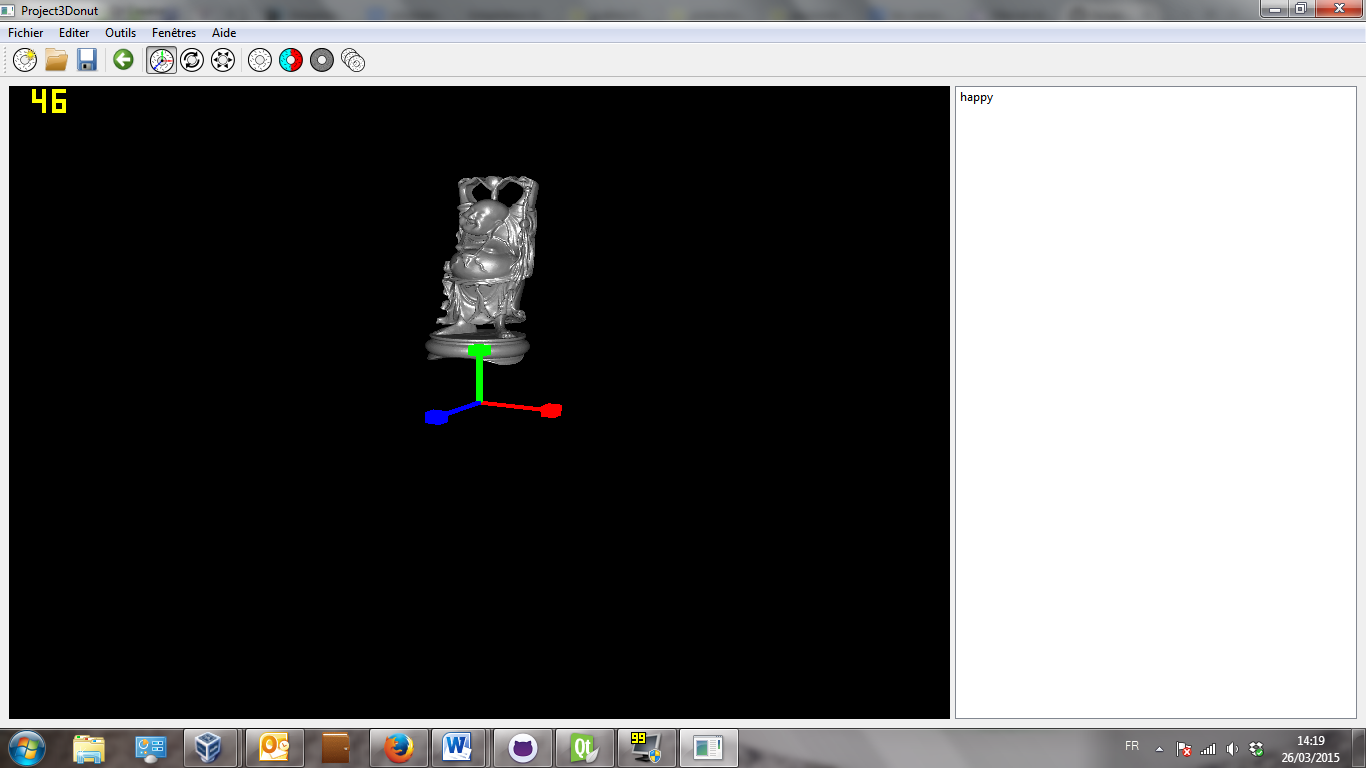
\includegraphics[scale=0.3]{happy_fps.png}
        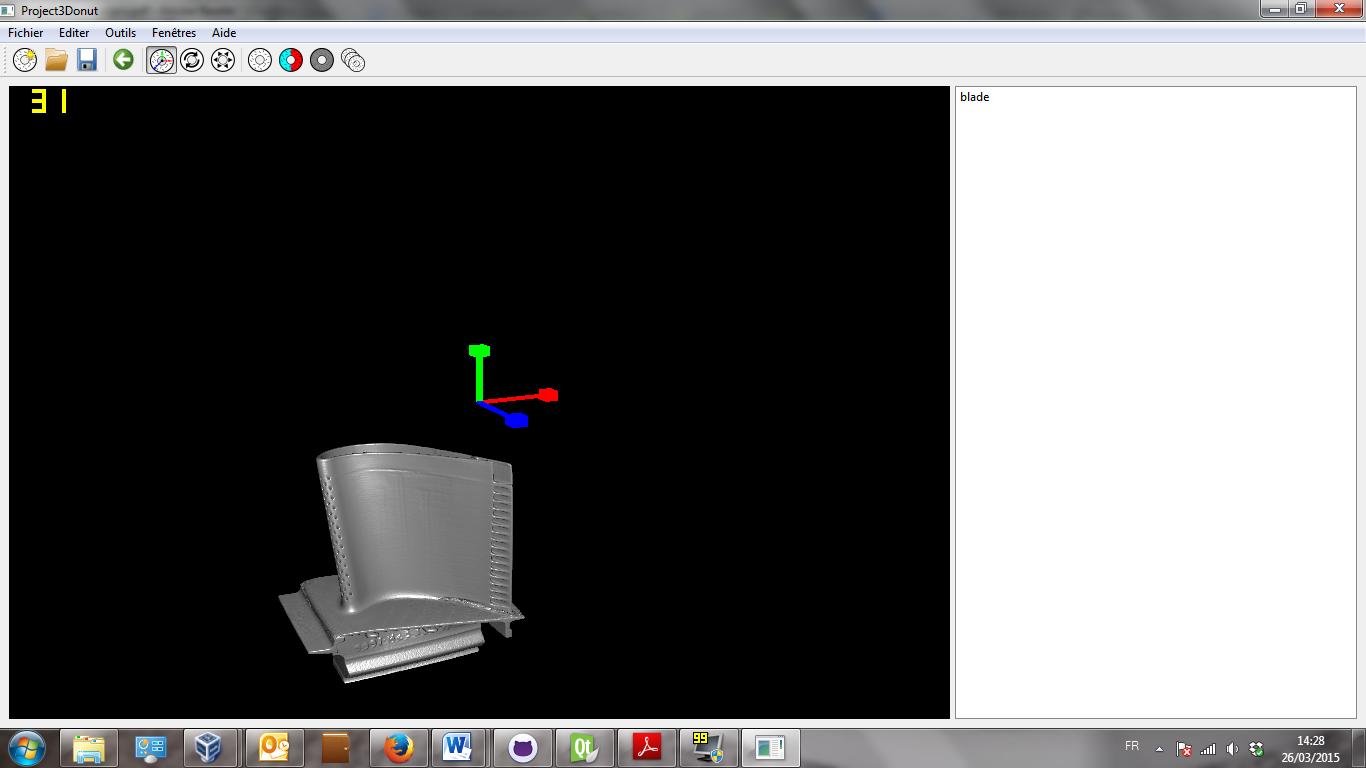
\includegraphics[scale=0.3]{blade_fps.png}
       	\caption{\label{fig:fps_windows_chipset} Test de fps sur une machine Windows avec chipset graphique\protect}
\end{figure}
[RESULTATS WINDOWS/LINUX/CHIPSET]
[RESULTAT SANS CHIPSET]

\paragraph{}
L'ensemble de ces tests auront permis de s'assurer de la conformité de notre projet au Cahier des charges. 
